\section{Categories: products, coproducts, and free objects}
\begin{ex}
    A \emph{pointed set} is a pair $(S,x)$ with $S$ a set and $x\in S$. A morphism of pointed sets $(S,x)\to (S', x')$ is a triple $(f,x,x')$, where $S\to S'$ is a function such that $f(x)=x'$. Show that pointed sets form a category.
\end{ex}

\begin{answer}
    Let $\mathcal{S}$ be the category and 4 objects of $\mathcal{S}$ are $(A,a)$, $(B,b)$, $(C,c)$, $(D,d)$. $f$, $g$ and $h$ are morphisms defined by $f:A\to B$, $g:B\to C$, $h:C\to D$ with $f(a)=b$, $g(b)=c$, $h(c)=d$.

    \begin{figure}[H]\centering
        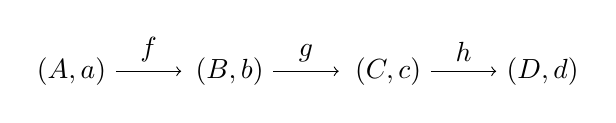
\begin{tikzpicture}
            \node [left] at (0,1) {$(A,a)$};
            \node [left] at (2,1) {$(B,b)$};
            \node [left] at (4,1) {$(C,c)$};
            \node [left] at (6,1) {$(D,d)$};
            \draw [->] (0,1)-- node [above, pos=0.5]{$f$}(0.83,1);
            \draw [->] (2,1)-- node [above, pos=0.5]{$g$}(2.83,1);
            \draw [->] (4,1)-- node [above, pos=0.5]{$h$}(4.83,1);
        \end{tikzpicture}
        \caption*{category $\mathcal{S}$}
    \end{figure}
    \[\mathrm{hom}(A,B)\times\mathrm{hom}(B,C)\to \mathrm{hom}(A,C)\]because $g\circ f:A\to C$ with $g(f(a))=g(b)=c=g\circ f(a)$. Similarly, $(h\circ g)\circ f=h\circ (g\circ f)$ with $(h\circ g)\circ f(a)=h\circ (g\circ f)(a)=d$. Take $1_{B}$ consist of those functions $i:B\to B$ with $i(b)=b$. Then $1_{B}\circ f=f$ and $g\circ 1_{B}=g$. So $\mathcal{S}$ is a category.
\end{answer}

$$ $$

\begin{ex}
    If $f:A\to B$ is an equivalence in a category $\mathcal{C}$ and $g:B\to A$ is the morphism such that $g\circ f=1_{A}$, $f\circ g=1_{B}$, show that $g$ is unique.
\end{ex}

\begin{answer}
    Assume there exist $g$ and $g'$ satisfies the condition.

    \begin{figure}[H]\centering
        \subfigure{
            \begin{minipage}[c]{0.3\linewidth}
                \centering
                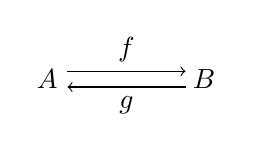
\begin{tikzpicture}
                    \node [left] at (0,1) {$A$};
                    \node [left] at (2,1) {$B$};
                    \draw [->] (0,1.1)-- node [above, pos=0.5]{$f$} (1.5,1.1);
                    \draw [<-] (0,0.9)-- node [below, pos=0.5]{$g$} (1.5,0.9);
                \end{tikzpicture}
            \end{minipage}
        }
        \subfigure{
            \begin{minipage}[c]{0.3\linewidth}
                \centering
                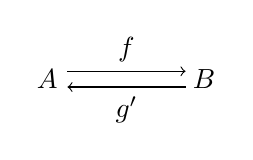
\begin{tikzpicture}
                    \node [left] at (0,1) {$A$};
                    \node [left] at (2,1) {$B$};
                    \draw [->] (0,1.1)-- node [above, pos=0.5]{$f$} (1.5,1.1);
                    \draw [<-] (0,0.9)-- node [below, pos=0.5]{$g'$} (1.5,0.9);
                \end{tikzpicture}
            \end{minipage}
        }
    \end{figure}
    So $g'\circ(f\circ g)=g'\circ 1_{B}=g'=(g'\circ f)\circ g=1_{A}\circ g =g$.
\end{answer}

$$ $$

\begin{ex}
    In the category $\mathcal{G}$ of groups, show that the group $G_{1}\times G_{2}$ together with the homomorphisms $\pi_{1}:G_{1}\times G_{2}\to G_{1}$ and $\pi_{2}:G_{1}\times G_{2}\to G_{2}$ is a product for $\{G_{1},G_{2}\}$.
\end{ex}

\begin{answer}
    Take $\tau_{1}:G_{1}\to G_{1}\times G_{2}$ as $\tau_{1}(g_{1})=(g_{1},e)$; $\tau_{2}:G_{2}\to G_{1}\times G_{2}$ as $\tau_{2}(g_{2})=(e,g_{2})$; $\pi_{1}:G_{1}\times G_{2}\to G_{1}$ as $\pi_{1}(g_{1},g_{2})=g_{1}$; $\pi_{2}:G_{1}\times G_{2}\to G_{2}$ as $\pi_{2}(g_{1},g_{2})=g_{2}$. Then

    \begin{figure}[H]\centering
        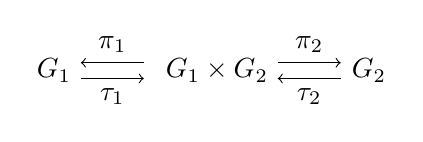
\begin{tikzpicture}
            \node [left] at (0,1) {$G_{1}$};
            \node [left] at (2.5,1) {$G_{1}\times G_{2}$};
            \node [left] at (4,1) {$G_{2}$};
            \draw [<-] (0,1.1)-- node [above, pos=0.5]{$\pi_{1}$} (0.8,1.1);
            \draw [->] (0,0.9)-- node [below, pos=0.5]{$\tau_{1}$} (0.8,0.9);
            \draw [->] (2.5,1.1)-- node [above, pos=0.5]{$\pi_{2}$} (3.3,1.1);
            \draw [<-] (2.5,0.9)-- node [below, pos=0.5]{$\tau_{2}$} (3.3,0.9);
        \end{tikzpicture}
    \end{figure}
    For any object $B$ such that

    \begin{figure}[H]\centering
        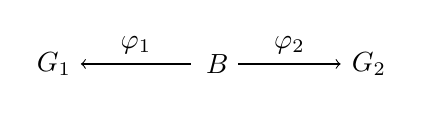
\begin{tikzpicture}
            \node [left] at (0,1) {$G_{1}$};
            \node [left] at (2,1) {$B$};
            \node [left] at (4,1) {$G_{2}$};
            \draw [<-] (0,1)-- node [above, pos=0.5]{$\varphi_{1}$} (1.4,1);
            \draw [->] (2,1)-- node [above, pos=0.5]{$\varphi_{2}$} (3.3,1);
        \end{tikzpicture}
    \end{figure}
    For any $x\in B$, define $f:B\to G_{1}\times G_{2}$ as $f(x)=(\varphi_{1}(x), \varphi_{2}(x))$. Then $\pi_{1}(f(x))=\varphi_{1}(x)$, $\pi_{1}\circ f=\varphi_{1}$, $\pi_{2}(f(x))=\varphi_{2}(x)$, $\pi_{2}\circ f=\varphi_{2}$. Thus
    
    \begin{figure}[H]\centering
        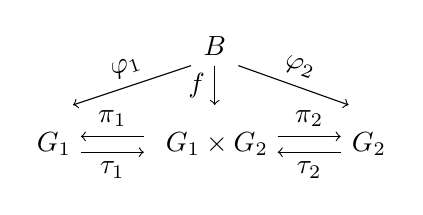
\begin{tikzpicture}
            \node [left] at (0,1) {$G_{1}$};
            \node [left] at (2.5,1) {$G_{1}\times G_{2}$};
            \node [left] at (4,1) {$G_{2}$};
            \draw [<-] (0,1.1)-- node [above, pos=0.5]{$\pi_{1}$} (0.8,1.1);
            \draw [->] (0,0.9)-- node [below, pos=0.5]{$\tau_{1}$} (0.8,0.9);
            \draw [->] (2.5,1.1)-- node [above, pos=0.5]{$\pi_{2}$} (3.3,1.1);
            \draw [<-] (2.5,0.9)-- node [below, pos=0.5]{$\tau_{2}$} (3.3,0.9);
            \node [above] at (1.7,2) {$B$};
            \draw [->] (1.7,2)-- node [left, pos=0.5]{$f$} (1.7,1.5);
            \draw [->] (1.4,2)-- node [above, pos=0.5, sloped]{$\varphi_{1}$} (-0.1,1.5);
            \draw [->] (2,2)-- node [above, pos=0.5, sloped]{$\varphi_{2}$} (3.4,1.5);
        \end{tikzpicture}
    \end{figure}
    Next we verify the uniqueness. If there exist $f$ and $f'$ satisfies the condition, \[\pi_{1}(f(x))=\pi_{1}(f'(x))=\varphi_{1}(x)\]\[\pi_{2}(f(x))=\pi_{2}(f'(x))=\varphi_{2}(x)\]Thus $f(x)=f'(x)$ for all $x\in B$, so $f=f'$.
\end{answer}

$$ $$

\begin{ex}
    In the category $\mathcal{A}$ of abelian groups, show that the group $A_{1}\times A_{2}$ together with the morphisms $\tau_{1}:A_{1}\to A_{1}\times A_{2}$ and $\tau_{2}:A_{2}\to A_{1}\times A_{2}$ is a coproduct of $\{A_{1}, A_{2}\}$.
\end{ex}

\begin{answer}
    Take $\tau_{1}:A_{1}\to A_{1}\times A_{2}$ as $\tau_{1}(a_{1})=(a_{1},e)$; $\tau_{2}:A_{2}\to A_{1}\times A_{2}$ as $\tau_{2}(a_{2})=(e,a_{2})$; $\pi_{1}:A_{1}\times A_{2}\to A_{1}$ as $\pi_{1}(a_{1},a_{2})=a_{1}$; $\pi_{2}:A_{1}\times A_{2}\to A_{2}$ as $\pi_{2}(a_{1},a_{2})=a_{2}$. Then

    \begin{figure}[H]\centering
        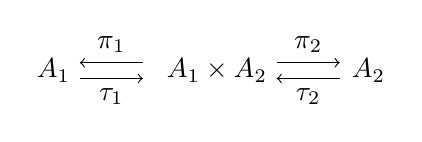
\begin{tikzpicture}
            \node [left] at (0,1) {$A_{1}$};
            \node [left] at (2.5,1) {$A_{1}\times A_{2}$};
            \node [left] at (4,1) {$A_{2}$};
            \draw [<-] (0,1.1)-- node [above, pos=0.5]{$\pi_{1}$} (0.8,1.1);
            \draw [->] (0,0.9)-- node [below, pos=0.5]{$\tau_{1}$} (0.8,0.9);
            \draw [->] (2.5,1.1)-- node [above, pos=0.5]{$\pi_{2}$} (3.3,1.1);
            \draw [<-] (2.5,0.9)-- node [below, pos=0.5]{$\tau_{2}$} (3.3,0.9);
        \end{tikzpicture}
    \end{figure}
    For any object $B$ such that

    \begin{figure}[H]\centering
        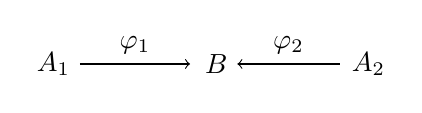
\begin{tikzpicture}
            \node [left] at (0,1) {$A_{1}$};
            \node [left] at (2,1) {$B$};
            \node [left] at (4,1) {$A_{2}$};
            \draw [->] (0,1)-- node [above, pos=0.5]{$\varphi_{1}$} (1.4,1);
            \draw [<-] (2,1)-- node [above, pos=0.5]{$\varphi_{2}$} (3.3,1);
        \end{tikzpicture}
    \end{figure}
    For any $(a_{1},a_{2})\in A_{1}\times A_{2}$, define $f:A_{1}\times A_{2}\to B$ as $f(a_{1},a_{2})=\varphi_{1}(a_{1})\varphi_{2}(a_{2})$. Then $f(\tau_{1}(a_{1}))=f(a_{1},e)=\varphi_{1}(a_{1})e=\varphi_{1}(a_{1})$, $f\circ \tau_{1}=\varphi_{1}$, $f(\tau_{2}(a_{2}))=f(e,a_{2})=e\varphi_{2}(a_{2})=\varphi_{2}(a_{2})$, $f\circ \tau_{2}=\varphi_{2}$.

    \begin{figure}[H]\centering
        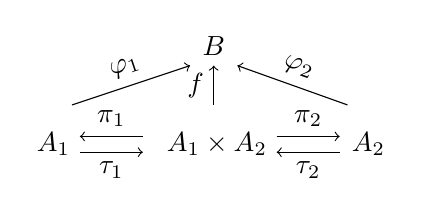
\begin{tikzpicture}
            \node [left] at (0,1) {$A_{1}$};
            \node [left] at (2.5,1) {$A_{1}\times A_{2}$};
            \node [left] at (4,1) {$A_{2}$};
            \draw [<-] (0,1.1)-- node [above, pos=0.5]{$\pi_{1}$} (0.8,1.1);
            \draw [->] (0,0.9)-- node [below, pos=0.5]{$\tau_{1}$} (0.8,0.9);
            \draw [->] (2.5,1.1)-- node [above, pos=0.5]{$\pi_{2}$} (3.3,1.1);
            \draw [<-] (2.5,0.9)-- node [below, pos=0.5]{$\tau_{2}$} (3.3,0.9);
            \node [above] at (1.7,2) {$B$};
            \draw [<-] (1.7,2)-- node [left, pos=0.5]{$f$} (1.7,1.5);
            \draw [<-] (1.4,2)-- node [above, pos=0.5, sloped]{$\varphi_{1}$} (-0.1,1.5);
            \draw [<-] (2,2)-- node [above, pos=0.5, sloped]{$\varphi_{2}$} (3.4,1.5);
        \end{tikzpicture}
    \end{figure}
    Next we verify the uniqueness. If there exist $f$ and $f'$ satisfies the condition, \[f(\tau_{1}(a_{1}))=f'(\tau_{1}(a_{1}))=f(a_{1},e)=f'(a_{1},e)\]\[f(\tau_{2}(a_{2}))=f'(\tau_{2}(a_{2}))=f(e,a_{2})=f'(e,a_{2})\]\[\begin{aligned}
        &f(\tau_{1}(a_{1}),\tau_{2}(a_{2}))=f(\tau_{1}(a_{1}))f(\tau_{2}(a_{2}))\\=&f'(\tau_{1}(a_{1}),\tau_{2}(a_{2}))=f'(\tau_{1}(a_{1}))f'(\tau_{2}(a_{2}))
    \end{aligned}\]
    so $f=f'$.
\end{answer}

$$ $$

\begin{ex}
    Every family $\{A_{i}|i\in I\}$ in the category of sets has a coproduct.
\end{ex}

\begin{answer}
    We examine $\bigcup\limits^{\cdot}A_{i}=\{(a,i)\in (\cup A_{i})\times I|a\in A_{i}\}$ which satisfies the condition. Define the morphism $\pi_{i}:A_{i}\to \bigcup\limits^{\cdot}A_{i}$ as $\pi_{i}(a)=(a,i)$. For any $B$ such that $\exists \varphi_{i}:A_{i}\to B$.
    
    \begin{figure}[H]\centering
        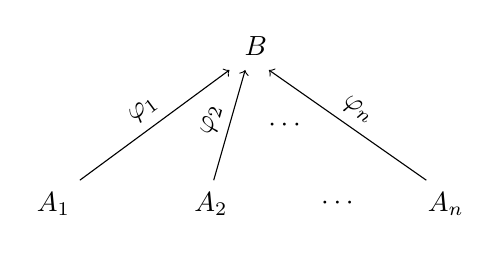
\begin{tikzpicture}
            \node [left] at (0,1) {$A_{1}$};
            \node [left] at (2,1) {$A_{2}$};
            \node [left] at (3.6,1) {$\cdots$};
            \node [left] at (5,1) {$A_{n}$};
            \node [left] at (2.5,3) {$B$};
            \draw [->] (0,1.3)-- node [above, pos=0.5, sloped]{$\varphi_{1}$} (1.9,2.7);
            \draw [->] (1.7,1.3)-- node [above, pos=0.5, sloped]{$\varphi_{2}$} (2.1,2.7);
            \draw [->] (4.4,1.3)-- node [above, pos=0.5, sloped]{$\varphi_{n}$} (2.4,2.7);
            \node [above] at (2.6,1.8) {$\cdots$};
        \end{tikzpicture}
    \end{figure}
    $\varphi(a)=x\in B$. Take $\varphi(a,i)=\varphi_{i}(a)$ defined on the subset of $\cup A_{i}\times I$, we can verify that the domain of $\varphi$ is $\bigcup\limits^{\cdot}A_{i}$. Then take $f=\varphi$, $f(\pi_{i}(a))=\varphi_{i}(a)$, $f\circ \pi_{i}=\varphi_{i}$.

    The uniqueness is obvious.
\end{answer}

$$ $$

\begin{ex}
    \begin{enumerate}[(a)]
        \item Show that in the category $\mathcal{S}_{*}$ of pointed sets product always exist; describe them.
        \item Show that in $\mathcal{S}_{*}$ every family of objects has a coproduct, describe the coproduct.
    \end{enumerate}
\end{ex}

\begin{answer}
    \begin{enumerate}[(a)]
        \item Define $\otimes$ as an operator between points and other elements in the pointed set. $\forall a\in A_{i}$, $a\otimes a_{i}=a_{1}\times a=a$. For a family of sets with their points $\{(A_{i},a_{i}|i\in I)\}$, consider $(A_{1}, A_{2}, \cdots, A_{n})=\{(a_{1}', a_{2}',\cdots, a_{n}')\}$. Define morphisms $\pi_{i}(a)=(a_{1}, a_{2},\cdots, a,\cdots, a_{n})$, $\pi_{i}:A_{i}\to (A_{1}, A_{2}, \cdots, A_{n})$.
        
        \begin{figure}[H]\centering
            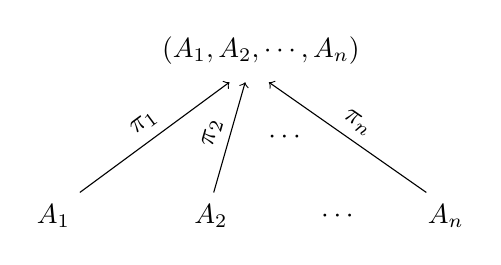
\begin{tikzpicture}
                \node [left] at (0,1) {$A_{1}$};
                \node [left] at (2,1) {$A_{2}$};
                \node [left] at (3.6,1) {$\cdots$};
                \node [left] at (5,1) {$A_{n}$};
                \node [above] at (2.3,2.8) {$(A_{1}, A_{2}, \cdots, A_{n})$};
                \draw [->] (0,1.3)-- node [above, pos=0.5, sloped]{$\pi_{1}$} (1.9,2.7);
                \draw [->] (1.7,1.3)-- node [above, pos=0.5, sloped]{$\pi_{2}$} (2.1,2.7);
                \draw [->] (4.4,1.3)-- node [above, pos=0.5, sloped]{$\pi_{n}$} (2.4,2.7);
                \node [above] at (2.6,1.8) {$\cdots$};
            \end{tikzpicture}
        \end{figure}
        For any $B$ such that $\exists \varphi_{i}:A_{i}\to B$.
    
        \begin{figure}[H]\centering
            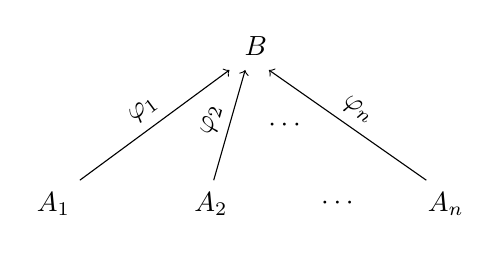
\begin{tikzpicture}
                \node [left] at (0,1) {$A_{1}$};
                \node [left] at (2,1) {$A_{2}$};
                \node [left] at (3.6,1) {$\cdots$};
                \node [left] at (5,1) {$A_{n}$};
                \node [left] at (2.5,3) {$B$};
                \draw [->] (0,1.3)-- node [above, pos=0.5, sloped]{$\varphi_{1}$} (1.9,2.7);
                \draw [->] (1.7,1.3)-- node [above, pos=0.5, sloped]{$\varphi_{2}$} (2.1,2.7);
                \draw [->] (4.4,1.3)-- node [above, pos=0.5, sloped]{$\varphi_{n}$} (2.4,2.7);
                \node [above] at (2.6,1.8) {$\cdots$};
            \end{tikzpicture}
        \end{figure}
        Take $f:(A_{1}, A_{2}, \cdots, A_{n})\to B$ as \[f(a_{1}',a_{2}',\cdots,a_{n}')=\varphi_{1}(a_{1}')\otimes\varphi_{2}(a_{2}')\otimes\cdots\otimes\varphi(a_{n}')\]Then $f\circ\pi_{i}(a)=f(a_{1},a_{2},\cdots,a,\cdots, a_{n})=\varphi_{1}(a_{1})\otimes\cdots\otimes\varphi_{i}(a)\otimes\cdots\otimes\varphi_{n}(a_{n})=\varphi_{i}(a)$. So $f\circ \pi_{i}=\varphi_{i}$.

        Next we verify the uniqueness. If there exist $f$ and $f'$ satisfies the condition. Then $\exists i\in I$ and $a\in A_{i}$ s.t. $f(a_{1},a_{2},\cdots,a,\cdots,a_{n})\neq f'(a_{1},a_{2},\cdots,a,\cdots,a_{n})$. But $f(\pi_{i}(a))=f'(\pi_{i}(a))$, so $f=f'$.
        \item The proof is similar to \textbf{Exercise 1.7.5}.
    \end{enumerate}
\end{answer}

$$ $$

\begin{ex}
    Let $F$ be a free object on a set $X(i:X\to F)$ in a concrete category $\mathcal{C}$. If $\mathcal{C}$ contains an object whose underlying set has at least two elements in it, then $i$ is an injective map of sets.
\end{ex}

\begin{answer}
    Assume $A\in\mathrm{obj}(\mathcal{C})$, $A$ has at least two elements and $X\xrightarrow{f} A$. $X\xrightarrow{i} F$ and $F$ is free on $X$, so there exists a morphism $\bar{f}$ s.t. $F\xrightarrow{\bar{f}}A$. If $\left| X \right|=1$, $i$ must be injective. For $\left| X \right| \geq 2$. Suppose $i$ is not injective. Take $x_{1}, x_{2}\in X$ and $i(x_{1})=i(x_{2})\in F$, $f(x_{1})=a_{1}$, $f(x_{2})=a_{2}$. $\bar{f}(i(x_{1}))=\bar{f}(i(x_{2}))=f(x_{1})=f(x_{2})=a_{1}=a_{2}$. That means all the elements in $A$ are identical. That's contradictory to the assumption.
\end{answer}

$$ $$

\begin{ex}
    Suppose $X$ is a set and $F$ is a free object on $X$ (with $i:X\to F$) in the category of groups. Prove that $i(X)$ is a set of generators for the group $F$.
\end{ex}

\begin{answer}
    Assume $G$ the subgroup of $F$ is the group generated by $i(X)$. Since $X\xrightarrow{i}G$ and $X\xrightarrow{i}F$, we can obtain unique morphism $\varphi$ such that $F\xrightarrow{\varphi}G$ and $\varphi \circ i=i$. 
    
    Consider morphism $1_{F}:F\to F$ which is the identical homomorphism. $F$ is free so $1_{F}$ is the unique homomorphism. Take $\subset:G\to F$ as a morphism defined as $\forall g\in G$, $\subset(g)=g$. Then
    
    \begin{figure}[H]\centering
        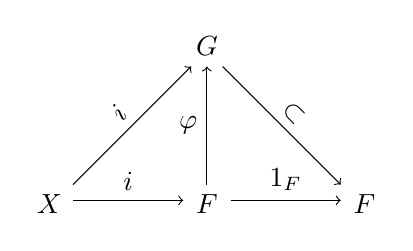
\begin{tikzpicture}
        \node [below] at (0,1) {$X$};
        \node [below] at (2,1) {$F$};
        \node [below] at (4,1) {$F$};
        \node [below] at (2,3) {$G$};
        \draw [->] (0.3,0.8)-- node [above, pos=0.5] {$i$} (1.7,0.8);
        \draw [->] (2.3,0.8)-- node [above, pos=0.5] {$1_{F}$} (3.7,0.8);
        \draw [->] (2,1)-- node [left, pos=0.5] {$\varphi$} (2,2.5);
        \draw [->] (0.3,1)-- node [above, pos=0.5, sloped] {$i$} (1.8,2.5);
        \draw [<-] (3.7,1)-- node [above, pos=0.5, sloped] {$\subset$} (2.2,2.5);
        \end{tikzpicture}
    \end{figure}
    $\subset\circ\varphi\circ i=1_{F}\circ i=i$ so $\subset\circ\varphi=1_{F}$. Thus $\subset$ is an epimorphism, $F\subset G$. So $F=G$ can be generated by $i(X)$.
\end{answer}